\section{Resultados}

A continuación, se presentan los resultados obtenidos durante la sesión de laboratorio para el estudio del contactor o conmutador electromagnético. El desarrollo experimental inició con el registro fotográfico del dispositivo y continuó con la toma de mediciones eléctricas.

\subsection{Registro Fotográfico del Contactor}
Como primera actividad en el laboratorio, se capturaron imágenes detalladas del dispositivo físico para documentar sus aspectos constructivos. A continuación, se presenta el registro fotográfico obtenido.

La Figura~\ref{fig:contactor_desarmado} muestra las piezas del contactor; de izquierda a derecha se tiene el núcleo magnético, la armadura móvil (o martillo), la carcasa inferior, la bobina de control y el resorte. Adicionalmente, se identificaron las espiras de sombra del contactor, tal como se muestra en la Figura~\ref{fig:espiras_sombra}. Por otra parte, al juntar el núcleo magnético con el martillo se identificaron los orificios que representan el entrehierro.

\begin{figure}[H]
    \centering
    \begin{subfigure}[b]{0.45\textwidth}
        \centering
        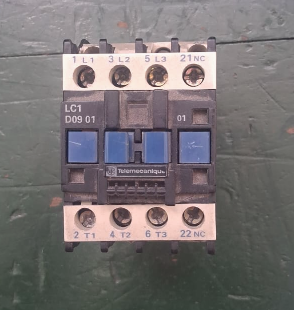
\includegraphics[width=\textwidth]{imagenes/contactor-experimento-cara-frontal.png}
        \caption{Vista frontal.}
        \label{fig:cara_frontal}
    \end{subfigure}
    \hfill
    \begin{subfigure}[b]{0.45\textwidth}
        \centering
        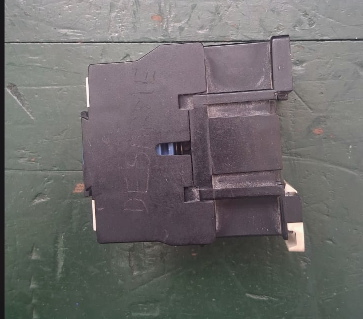
\includegraphics[width=\textwidth]{imagenes/contactor-experimento-cara-lateral.png}
        \caption{Vista lateral.}
        \label{fig:cara_lateral}
    \end{subfigure}
    \caption{Vistas frontal y lateral del contactor bajo estudio.}
    \label{fig:vistas_contactor}
\end{figure}

\begin{figure}[H]
    \centering
    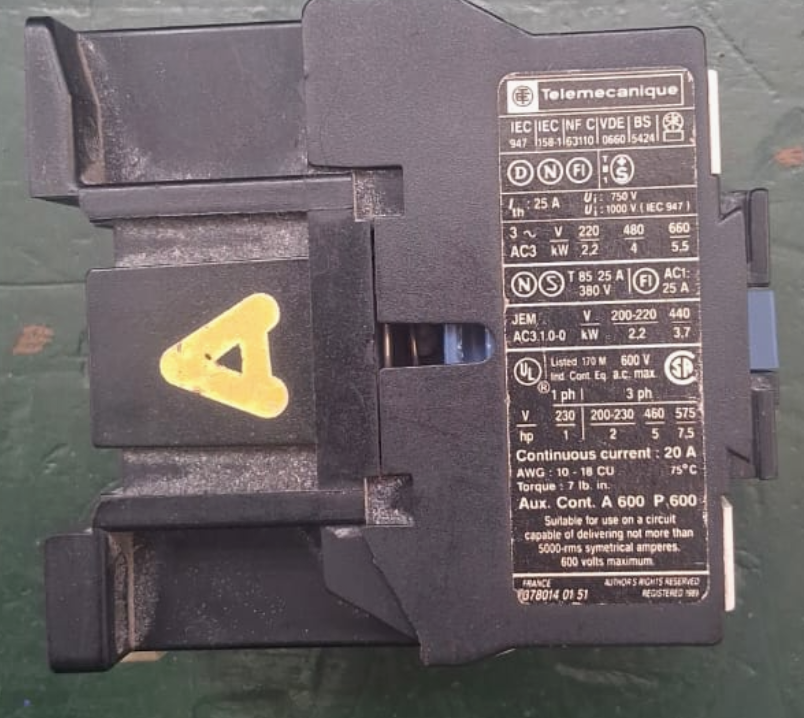
\includegraphics[width=0.6\textwidth]{imagenes/contactor-experimento-placa-datos.png}
    \caption{Placa de datos técnicos del fabricante.}
    \label{fig:placa_datos}
\end{figure}

\begin{figure}[H]
    \centering
    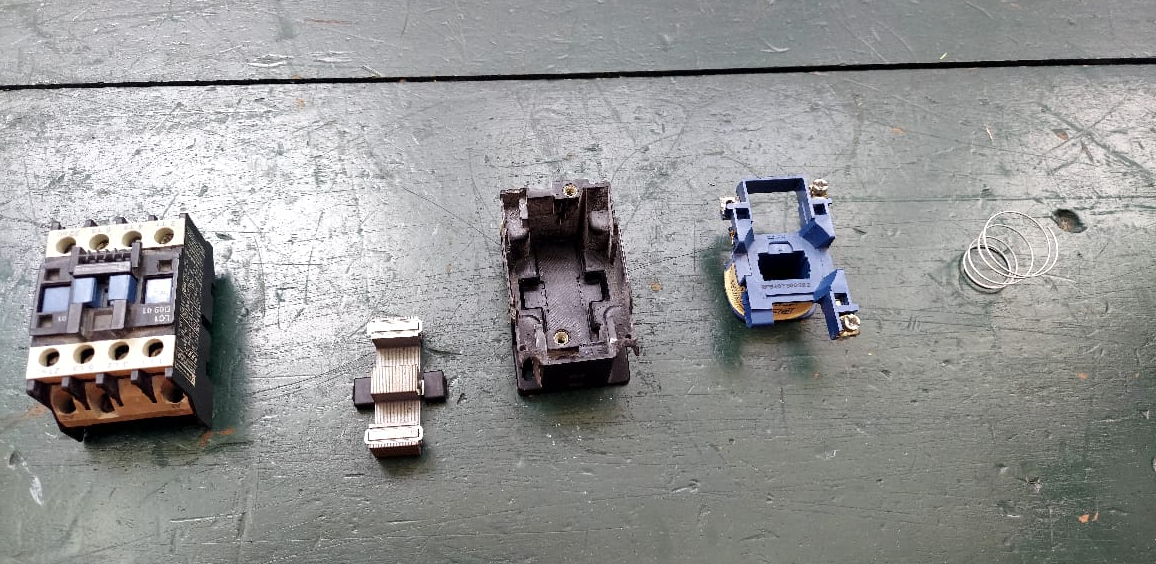
\includegraphics[width=0.85\textwidth]{imagenes/contactor-experimento-desarmado.png}
    \caption{Vista detallada del contactor desarmado, mostrando sus componentes internos.}
    \label{fig:contactor_desarmado}
\end{figure}

\begin{figure}[H]
    \centering
    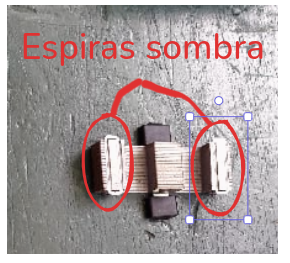
\includegraphics[width=0.6\textwidth]{imagenes/espiras-sombra.png}
    \caption{Detalle de las espiras de sombra en el núcleo del contactor.}
    \label{fig:espiras_sombra}
\end{figure}

\subsection{Mediciones del Contactor 1}
En la Tabla~\ref{tab:contactor_1} se muestran las mediciones obtenidas para el primer contactor ensayado, incluyendo sus incertidumbres asociadas de acuerdo con la precisión de los instrumentos de medición empleados.

\begin{table}[H]
    \centering
    \caption{Tabla de mediciones para el Contactor 1.}
    \label{tab:contactor_1}
    \begin{tabular}{lcc}
        \toprule
        \textbf{Parámetro} & \textbf{Placa (Fabricante)} & \textbf{Medición} \\
        \midrule
        Corriente de llamada & --- & $\num{0,18} \pm \num{0,005}$ \si{\ampere} \\
        Corriente de mantenimiento & --- & $\num{0,011} \pm \num{0,001}$ \si{\ampere} \\
        Tensión de mantenimiento & --- & $\num{188} \pm \num{2}$ \si{\volt} \\
        Tensión mínima de operación & --- & $\num{145} \pm \num{2}$ \si{\volt} \\
        Corriente de operación nominal\textsuperscript{*} & --- & $\num{0,02} \pm \num{0,001}$ \si{\ampere} \\
        \bottomrule
    \end{tabular}
    \begin{flushleft}
        \footnotesize
        \textsuperscript{*} La corriente de operación nominal se especifica inmediatamente debajo de la primera sección de la hoja de toma de datos. \\
        \textbf{Nota:} Se incluye una anotación manuscrita en la hoja original que indica: ``Pinza Amperimétrica Ref $\rightarrow$ \num{0,18} / \num{0,014}''.
    \end{flushleft}
\end{table}

\subsection{Mediciones del Contactor 2}
En la Tabla~\ref{tab:contactor_2} se detallan las mediciones y parámetros registrados para el segundo contactor ensayado.

\begin{table}[H]
    \centering
    \caption{Tabla de mediciones para el Contactor 2.}
    \label{tab:contactor_2}
    \begin{tabular}{lc}
        \toprule
        \textbf{Parámetro} & \textbf{Medición} \\
        \midrule
        Corriente de llamada & $\num{2,94} \pm \num{0,01}$ \si{\ampere} \\
        Corriente de mantenimiento & $\num{0,26} \pm \num{0,01}$ \si{\ampere} \\
        Tensión de mantenimiento & $\num{54} \pm \num{2}$ \si{\volt} \\
        Tensión mínima de operación & $\num{96} \pm \num{2}$ \si{\volt} \\
        \bottomrule
    \end{tabular}
\end{table}